\documentclass{scrartcl}
\title{Sprawozdanie 1 \\ Przetwarzanie równoległe}
\subtitle{Mnożenie macierzy porównanie efektywności metod –\\
3 pętle - kolejność pętli: jki,\\
6 pętli - kolejność pętli: zewnętrznych ijk, wewnętrznych: ikj, podział pracy przed pętlą 1.}
\date{2018-05-13}
\author{Bartosz Nawrotek, Krystian Hoczkiewicz \\
Prowadzący: dr inż. Rafał Walkowiak}

\usepackage{float}
\usepackage[utf8]{inputenc}
\usepackage{mathtools}
\usepackage{amssymb}
\usepackage[T1]{fontenc}
\usepackage{listings}
\usepackage{color}
\usepackage{geometry}
 \geometry{
 a4paper,
 total={170mm,257mm},
 left=20mm,
 top=20mm,
 }
\lstdefinestyle{mystyle}{
    backgroundcolor=\color{backcolour},   
    commentstyle=\color{codegreen},
    keywordstyle=\color{codeblue},
    numberstyle=\tiny\color{codegray},
    stringstyle=\color{codepurple},
    basicstyle=\footnotesize,
    breakatwhitespace=false,         
    breaklines=true,                 
    captionpos=b,                    
    keepspaces=true,                 
    numbers=left,                    
    numbersep=5pt,                  
    showspaces=false,                
    showstringspaces=false,
    showtabs=false,                  
    tabsize=2
}

\definecolor{codegreen}{rgb}{0,0.6,0}
\definecolor{codeblue}{rgb}{0,0,0.6}
\definecolor{codegray}{rgb}{0.5,0.5,0.5}
\definecolor{codepurple}{rgb}{0.58,0,0.82}
\definecolor{backcolour}{rgb}{0.95,0.95,0.92}

\usepackage{graphicx}
\graphicspath{ {img/}{img/figures/}}
\newcommand\tab[1][1cm]{\hspace*{#1}}
\lstset{style=mystyle}


\begin{document}
\maketitle
\section{Wstęp}
\paragraph{}Celem sprawozdania jest analiza wraz z porównaniem efektywności dwóch metod mnożenia macierzy w wersji równoległej oraz sekwencyjnej:
\begin{itemize}
\item {3 pętle w kolejności jki}
\item {6 pętli w kolejności zewnętrznych ijk, wewnętrznych ikj z podziałem pracy przed pierwszą pętlą}
\end{itemize}
\paragraph{}Wynikiem mnożenia jest macierz $R$, czynnikami macierze $A, B$. Iloczyn jest liczony wg poniższego wzoru:
\begin{equation}
R_{i, j} = \sum_{k = 1}^{n}{A_{i, k}B_{k, j}}
\end{equation}
gdzie $n$ jest ilością wierszy macierzy kwadratowych $A$ oraz $B$.
Do przeprowadzenia pomiarów korzystano z oprogramowania Code XL oraz do pomiaru czasu działania algorytmu biblioteka time.h.
\section{Analiza algorytmów oraz dyrektyw Open MP}
\subsection{Metoda 3 pętlowa JKI}
\begin{lstlisting}[language=C++, caption={Metoda trzypętlowa}]
void multiply_matrices_JKI()
{
        // mnozenie macierzy 
#pragma omp parallel for 
	for (int j = 0 ; j < COLUMNS ; j++)
      	    for (int k = 0 ; k < COLUMNS ; k++) 
                  for (int i = 0 ; i < ROWS ; i++) 
                        matrix_r[i][j]+= matrix_a[i][k] * matrix_b[k][j] ;              
}
\end{lstlisting}
\paragraph{}Jak widać metoda 3 pętlowa charakteryzuje się złożonością $O(n^3)$, gdzie $COLUMNS = ROWS = n$ dla macierzy kwadratowych. W sekwencyjnej metodzie 3 pętlowej wykorzystany został ten sam kod wraz z wyłączoną obsługą dyrektyw OpenMP. W wersji równoległej następuje przydział pracy przed pierwszą pętlą. Powoduje to statyczny podział pracy wg następującego wzoru:
\begin{equation}
j = <id \frac{COLUMNS}{4}, (id + 1)\frac{COLUMNS}{4} - 1>,
j \in \mathbb{Z}
\end{equation}
gdzie $j$ oznacza numer przydzielonej iteracji do procesora o numerze $id \in \{0, 1, 2, 3\}$ dla COLUMNS podzielnego na 4.
\subsection{Metoda 6 pętlowa IJK-IKJ}
\begin{lstlisting}[language=C++, caption={Metoda sześciopętlowa}]
void multiply_matrices_IJK_IKJ()
{
	int r = 10;
	#pragma omp parallel for
	for (int i = 0; i < ROWS; i+=r) {
		for (int j = 0; j < COLUMNS; j+=r) {
			for (int k = 0; k < COLUMNS; k+=r) {
				for (int ii = i; ii < i + r; ii++) {
					for (int kk = k; kk < k + r; kk++) {
						for (int jj = j; jj < j + r; jj++) {
						matrix_r[ii][jj] += matrix_a[ii][kk] * matrix_b[kk][jj];
						}
					}
				}
			}
		}
	}
}
\end{lstlisting}
\paragraph{}Metoda 6 pętlowa wykazuje się tą samą złożonością obliczeniową co metoda 3 pętlowa. Wykorzystanie jej ma jednak wpływ na prędkość przetwarzania ze względu na budowę systemu obliczeniowego. Korzysta on z pamięci cache oraz bufora translacji, które aby optymalnie wykorzystać, należy zapewnić odpowiednie warunki przetwarzania, jak lokalność przestrzenna oraz czasowa.
\subsection{Analiza poprawności algorytmów}
\paragraph{}Oba algorytmy w wersji sekwencyjnej są poprawne, ze względu na definicję mnożenia macierzy. W wersji równoległej również, ze względu na to, że każdy proces korzysta z innej, rozłącznej części macierzy wynikowej. Nie jest wymagana żadna dodatkowa metoda synchronizacji.
\subsection{Efektywność - synchronizacja}
\paragraph{}Jak było nadmienione w punkcie 2.1 oraz 2.2, obie metody cechują się tą samą złożonością obliczeniową. Jednak różnice efektywności mogą być znaczne ze względu na kolejność dostępu do danych z poszczególnych macierzy. Spodziewamy się prawie 4 krotnego przyspieszenia przetwarzania przy użyciu metod w wersji równoległej w stosunku do wersji sekwencyjnej ze względu na niski koszt synchronizacji (przydział pracy statyczny przed pętlą zewnętrzną oraz synchronizacja na końcu działania funkcji).
\newpage
\subsection{False sharing}
\paragraph{}Jest to zjawisko, które może wystąpić tylko w przypadku przetwarzania równoległego. W metodzie równoległej 3 pętlowej zjawisko może wystąpić na krańcach przydzielonych obszarów macierzy $R$. Nie powinno jednak mieć to większego wpływu na czas przetwarzania ze względu na stosunkowo niewielkie fragmenty macierzy, gdzie zjawisko ma możliwość się pojawić.
W metodzie równoległej 6 pętlowej zjawisko również może wystąpić na granicy ostatniego wiersza przydzielonego do danego procesora oraz pierwszego wiersza przydzielonego do kolejnego procesora. W tym wypadku, będzie prawdopodobnie niezauważalne, bo dla całej macierzy występują tylko 4 potencjalne miejsca wystąpienia tego zjawiska niezależnie od wielkości instancji.
\subsection{Lokalność dostępu do danych}
\paragraph{}Macierze deklarowane są jako tablice dwuwymiarowe, co implikuje przechowywanie ich w pamięci jako pojedyncza linia. Niesie to za sobą możliwość analizy lokalności dostępu do danych.
\begin{figure}[H]
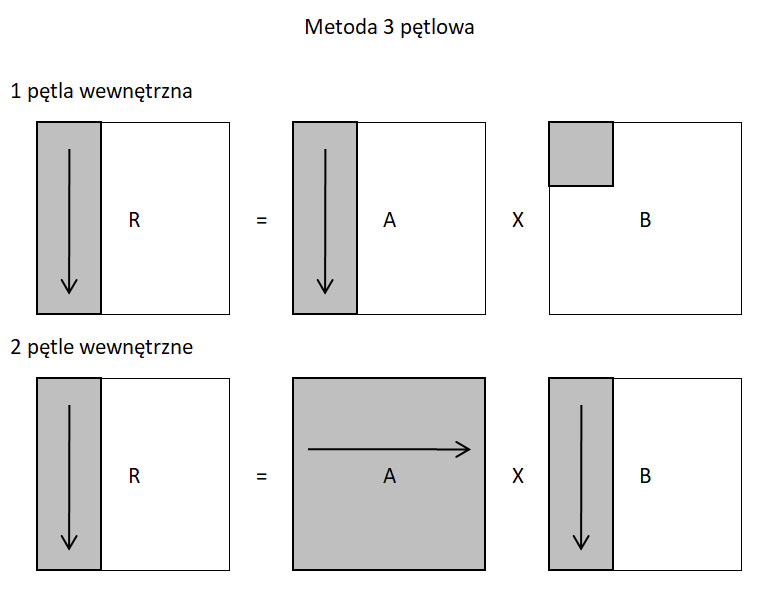
\includegraphics[width=\textwidth]{3petlowa.png}
\caption{Metoda 3 pętlowa JKI}
\end{figure}
\paragraph{}
Dla metody 3 pętlowej biorąc pod uwagę iteracje wewnętrznej pętli można wyciągnąć następujące wnioski dla poszczególnych macierzy: \\
\begin{itemize}
\item R - brak lokalności przestrzennej ani czasowej
\item A - brak lokalności przestrzennej ani czasowej
\item B - lokalność czasowa
\end{itemize}
\paragraph{}Natomiast dla dwóch pętli wewnętrznych:
\begin{itemize}
\item R - brak lokalności przestrzennej ani czasowej
\item A - lokalność przestrzenna, brak lokalności czasowej ze względu na odczyt danych w poszczególnych kolumnach. (kolejne czytane komórki mają oddalone adresy o $n$)
\item B - brak lokalności przestrzennej ani czasowej
\end{itemize}
\paragraph{}Braki lokalności spowodowane są iterowaniem po kolejnych elementach w kolumnach poszczególnych macierzy. Powodować to będzie znaczne spadki efektywności działania algorytm.
\begin{figure}[H]
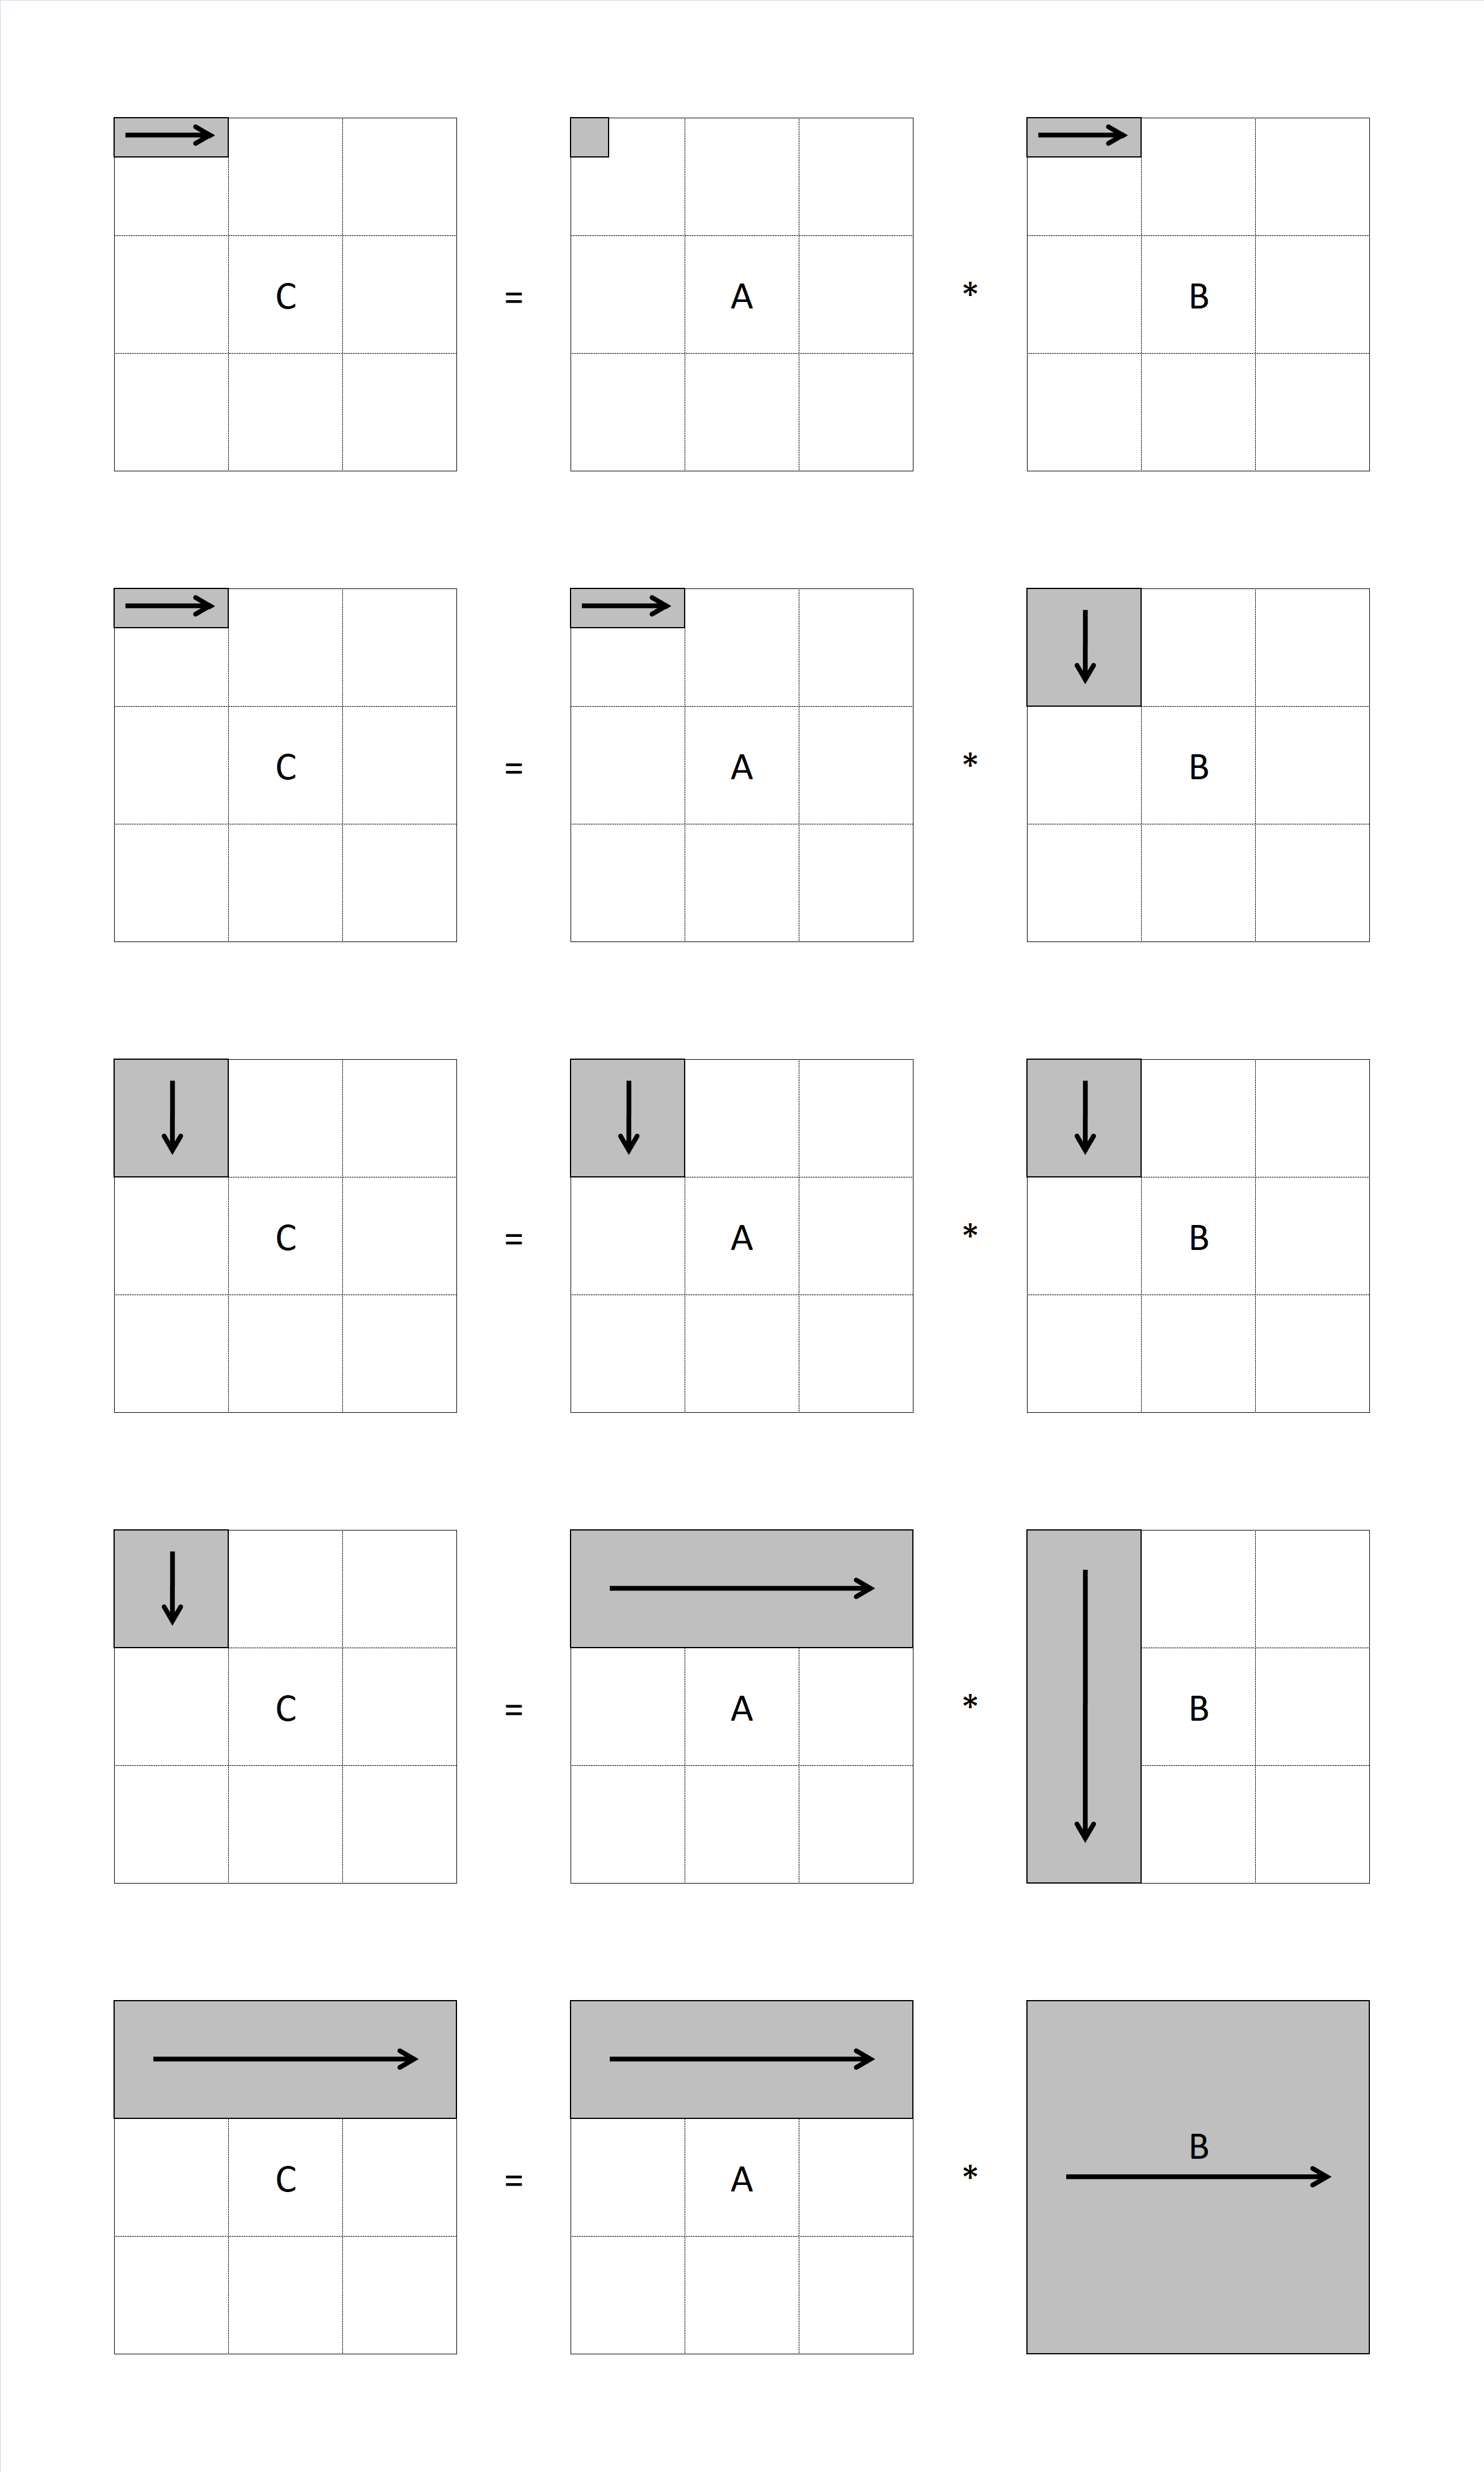
\includegraphics[width=\textwidth]{6petlowa.png}
\caption{Metoda 6 pętlowa IJK-IKJ}
\end{figure}
\paragraph{Uzasadnienie wielkości instancji} Aby zapewnić lokalność czasową przetwarzania należy spełnić poniższy warunek:
\begin{equation}
4N ^ 2 + 128 [B] <= 8192 [kB]
\end{equation}
\paragraph{}Pierwszy człon wynika z rozmiaru macierzy $A$. Człon drugi jest sumą pamięci potrzebnej do przechwania macierzy $B$ oraz $R$, na każdy element macierzy potrzebne jest jedno słowo w pamięci podręcznej o wielkości 64B. Suma tych dwóch człownów musi mieścić się w pamięci podręcznej o rozmiarze 8MB. \\
\begin{equation}
N <= 1431
\end{equation}
W związku z powyższym dowiadujemy się, że dla zadanej wielkości macierzy większej niz 1431 tracimy lokalność czasową.\\
\\
Aby zapewnić lokalność przestrzenną zdefiniowaną jako zapewnienie jednokrotnego uzupełnienia odwzorowania strony na ramkę pamięci dla $N > W_{ram}$, gdzie $W_{ram}$ jest wielkością ramki pamięci należy spełnić następujący warunek:
\begin{equation}
4N ^ 2 + 8192 N <= 550 * 4096 [B]
\end{equation}
\paragraph{}Pierwszy człon wynika z wielkości macierzy A, drugi z faktu, że na każdy element macierzy potrzebne jest zachowanie całej strony pamięci. Powyższa suma powinna mieścić się w buforze translacji o wielkości $550 * 4096[B]$.
\paragraph{}
Dla metody 6 pętlowej [1]:
\begin{itemize}
\item lokalność przestrzenna oraz czasowa
\item lokalność przestrzenna
\item lokalność przestrzenna oraz czasowa
\end{itemize}
[2]
\begin{itemize}
\item lokalność przestrzenna oraz czasowa
\item lokalność przestrzenna oraz czasowa
\item lokalność przestrzenna oraz czasowa
\end{itemize}
\subsection{Przydział pracy do wątków}
\paragraph{}Użycie dyrektywy Open MP "\#pragma omp parallel for" sprawia, że przydział pracy do wątków jest równomierny jeżeli jest to możliwe. Taki przydział występuje gdy liczba iteracji jest podzielna przez liczbę procesorów. W przeciwnym wypadku pozostałe iteracje (ich ilość jest równa reszcie z dzielenia liczby iteracji na liczbę procesorów)jest rozdzielana między wątkami. W tym wypadku możliwe jest zaobserwowanie nieznacznego spadku efektywności działającego algorytmu.
//TODO OBRAZKI
\section{Analiza przetwarzania}
\subsection{Prezentacja miar i jakości przetwarzania}
\paragraph{}
 Nazwa instancji - składa się na nią rozmiar macierzy, rozmiar instancji (w metodzie 6 pętlowej) oraz typ metody (3 lub 6 pętlowa).
\subsection{Metoda 3 pętlowa JKI}
\subsubsection{Sekwencyjnie}
\subsubsection{Równolegle}
\subsection{Metoda 6 pętlowa IJK-IKJ}
\subsubsection{Sekwencyjnie}
\subsubsection{Równolegle}
\section{Określenie zakresu zbieranych miar efektywności}
\section{Analiza pomiarów}
\subsection{Metoda 3 pętlowa JKI}
\paragraph{Czas obliczeń.} Na poniższym wykresie widać zależność między czasem obliczeń, a rozmiarem instancji. Potwierdza to złożoność zaproponowanego algorytmu równą $O(n^{3})$. W dodatku różnice czasów wykonań metody sekwencyjnej oraz równoległej pokazują, że dla małych instancji problemu zastosowanie algorytmu równoległego nie musi być odpowiednie, jednak możliwości algorytmów równoległych uwidaczniają się przy większych rozmiarach instancji.
\begin{figure}[H]
\includegraphics{Tobl3.png}\\
\end{figure}
\paragraph{Prędkość obliczeń.} Wykres prędkości obliczeń w metodzie 3 pętlowej świadczy natomiast o spadku efektywności zastosowanego algorytmu dla kolejnych rozmiarów instancji w obu metodach. Powody spadku efektywnosci zostaną wymienione w dalszej części sprawozdania.
\begin{figure}[H]
\includegraphics{Predkosc3.png}\\
\end{figure}
\paragraph{Instrukcje na cykl.} Wskaźnik \textbf{IPC} oznacza średnią liczbę instrukcji kodu asemblera przypadającą na cykl pracy procesora. Jak widać, dla metody 3 pętlowej przy rozmiarach instancji od $n = 256$ następuje gwałtowny spadek wartości wskaźnika, świadczy to o obecności czynników zmniejszających efektywność, takich jak słaba przestrzenna lub czasowa lokalność dostępów do pamięci.
\begin{figure}[H]
\includegraphics{IPC3.png}\\
\end{figure}
\paragraph{Stosunek braku trafień do L2 DTLB.} Na wykresie można zauważyć osiągnięcie stusunku braku trafień bliskiego $1$ już dla rozmiaru instancji $n = 512$, potwierdza to przewidywania dotyczące słabej lokalności przestrzennej dostępów do pamięci. Implikuje to znaczny spadek efektywności przetwarzania.
\begin{figure}[H]
\includegraphics{SBTDPPL33.png}\\
\end{figure}
\paragraph{Wskaźnik braku trafień do pp L3.} Wskaźnik został policzony wg wzoru: $PPL3\ miss\ rate = L3\ miss / Data\ access$. Dla $Data access = 0$ przyjęto, że wartość wskaźnika bedzie równa 0. Wartosci wskaźnika wskazują na niską lokalność czasową dostępów do pamięci. Dla małych rozmiarów instancji wskaźnik ma wartość 0 ze względu na fakt, że macierze są przetrzymywane w pamięci podręcznej od chwili ich inicjalizacji.
\begin{figure}[H]
\includegraphics{L3MissRate3.png}
\end{figure}
\paragraph{Przyspieszenie} Przyspieszenie osiąga wartość ponad $3.5$ od instancji o rozmiarze $n = 512$, świadczy to o tym, że problem jest łatwy do zrównoleglenia
\begin{figure}[H]
\includegraphics{Przyspieszenie3.png}
\end{figure}
\paragraph{Koszt synchronizacji} Koszt synchronizacji maleje wraz z rozmiarem instancji. Jest to zrozumiałe ze względu na fakt, że istnieje tylko jeden punkt synchronizacji wątków niezależnie od rozmiaru instancji.
\begin{figure}[H]
\includegraphics{Synchro3.png}
\end{figure}

\subsection{Metoda 6cio pętlowa}

\paragraph{Czas obliczeń.} Wykres czasu obliczeń w metodzie 6-cio pętlowej również wskazuje na złożoność obliczeniową problemu. Można zaobserwować również różnice w czasie obliczeń w zależności od wielkości parametru $r$. Jest ona spowodowana zajmowaniem przez kolejne podmacierze różnej ilości miejsca w pamięci podręcznej. W dalszej części sprawozdania przyjmujemy, że w nazwie instancji metody sześciopętlowej znajdują się odpowiednio $n$ oraz $r$ oddzielone separatorem '\_'
\begin{figure}[H]
\includegraphics{Tobl6.png}
\end{figure}

\paragraph{Prędkość obliczeń.} Dla metody 6-cio pętlowej prędkość obliczeń ulega niewielkim wahaniom w zależnosci od rozmiaru instancji, co pokazuje, że zastosowanie algorytmu 6-cio pętlowego pozwala poprawić lokalność przestrzenną lub czasową dostępów. Dla metody równoległej w zależności od wielkości parametru $r$ prędkość obliczeń ulega dużej zmianie. Najlepsze wyniki zostały uzyskane dla $r = 64$, następnie wraz ze wzrostem $r$, prędkość zaczyna maleć. Jest to spowodowane utratą czasowej lokalności dostępów do pamięci ze względu na zajmowanie przez podmacierz dużej ilości miejsca w pamięci podręcznej. Z drugiej jednak strony dla wielkości $r = 16$ również następuje spadek prędkości ze względu na częste odwołania do pp, przez co musi być ona częściej aktualizowana. Dla metody sekwencyjnej najlepszą mierzoną wartością r było 16, różnica może wynikać z tego, że dla wielu procesorów lokalnoś czasowa w ramach pętli czwartej wewnętrznej pozwala na wielokrotne używanie kolumny macierzy B przez wszystkie procesory.
\begin{figure}[H]
\includegraphics{Predkosc6.png}\\
\end{figure}

\paragraph{Instrukcje na cykl.} W odróżnieniu od metody 3 pętlowej wartość wskaźnika IPC utrzymuje podobną wartość w zależności od rozmiaru instancji, co wskazuje na obniżenie wpływu czynników obniżających efektywność przetwarzania kodu
\begin{figure}[H]
\includegraphics{IPC6.png}\\
\end{figure}

\paragraph{Stosunek braku trafień do L2 DTLB.} Dla metody 6-cio pętlowej przy odpowiednim doborze parametru $r$ można zapewnić lokalność przestrzenną dostępu do danych. W przypadku wybranych wartości $r$ udaje się zachować lokalność przestrzenną dla $r \in \{64, 128, 256\}$. TODO
\begin{figure}[H]
\includegraphics{SBTDPPL36.png}\\
\end{figure}

\paragraph{Wskaźnik braku trafień do pp L3.} W większości przypadków udało się utrzymać wskaźnik braku trafień do pp L3 na niskim poziomie, co wskazuje na to, że przy odpowiednim doborze parametru $r$ zachowujemy również lokalność czasową odwołań. Wyjątki widoczne na wykresie wynikają z nie mieszczenia się w pamięci podręcznej obszarów wynikających z wielkości podmacierzy oraz z częstego odwoływania się pp co może powodować, częstą wymianę danych w pp.
\begin{figure}[H]
\includegraphics{L3MissRate6.png}
\end{figure}

\paragraph{Przyspieszenie} Uzyskane wyniki przyspieszenia pozwalają stwierdzić, że dla metody 6-cio pętlowej również można osiągnąć wysoki stopień zrównoleglenia Skrajnie niskie wartości przyspieszenia wynikają z braku lokalności dostępów w metodzie równoległej, przy zachowaniu lokalności w metodzie sekwencyjnej. Niestety nie zostało to pokazane na poprzednich wykresach ze względu na mały rozmiar instancji, który nie pozwalał na przekroczenie dobranego progu zliczania.
\begin{figure}[H]
\includegraphics{Przyspieszenie6.png}
\end{figure}

\paragraph{Koszt synchronizacji} TODO
\begin{figure}[H]
\includegraphics{Synchro6.png}
\end{figure}

\section{Wnioski}
\end{document}